\section{Experimental Evaluation}
\label{sec:experiments}

\subsection{Robustness analysis of tolerance graphs}
\begin{table}[ht]
\caption{Robustness summary across $\tau$ (tolerance threshold)}
\centering
\begin{tabular}{lrrrr}
\toprule
$\tau$ & \#edges & \#components & largest comp & \#cliques \\
\midrule
0.75 & 1 & 40558 & 2 & 1 \\
0.70 & 4 & 40555 & 2 & 4 \\
0.65 & 47 & 40512 & 3 & 47 \\
0.60 & 355 & 40204 & 3 & 355 \\
0.55 & 1800 & 38765 & 8 & 1790 \\
0.50 & 5643 & 34977 & 30 & 5533 \\
0.45 & 15003 & 26050 & 357 & 13554 \\
\bottomrule
\end{tabular}
\label{tab:robustness}
\end{table}

\subsection{Clique and community statistics}
Figure~\ref{fig:clique_dist} shows the clique size distribution; Figure~\ref{fig:louvain_dist} and Figure~\ref{fig:leiden_dist} show community size distributions for Louvain and Leiden respectively.
\begin{figure}[ht]
\centering

\includegraphics[width=0.48\textwidth]{figures/clique_size_distribution.png}
\caption{Clique size distribution.}
\label{fig:clique_dist}
\end{figure}
\begin{figure}[ht]
\centering
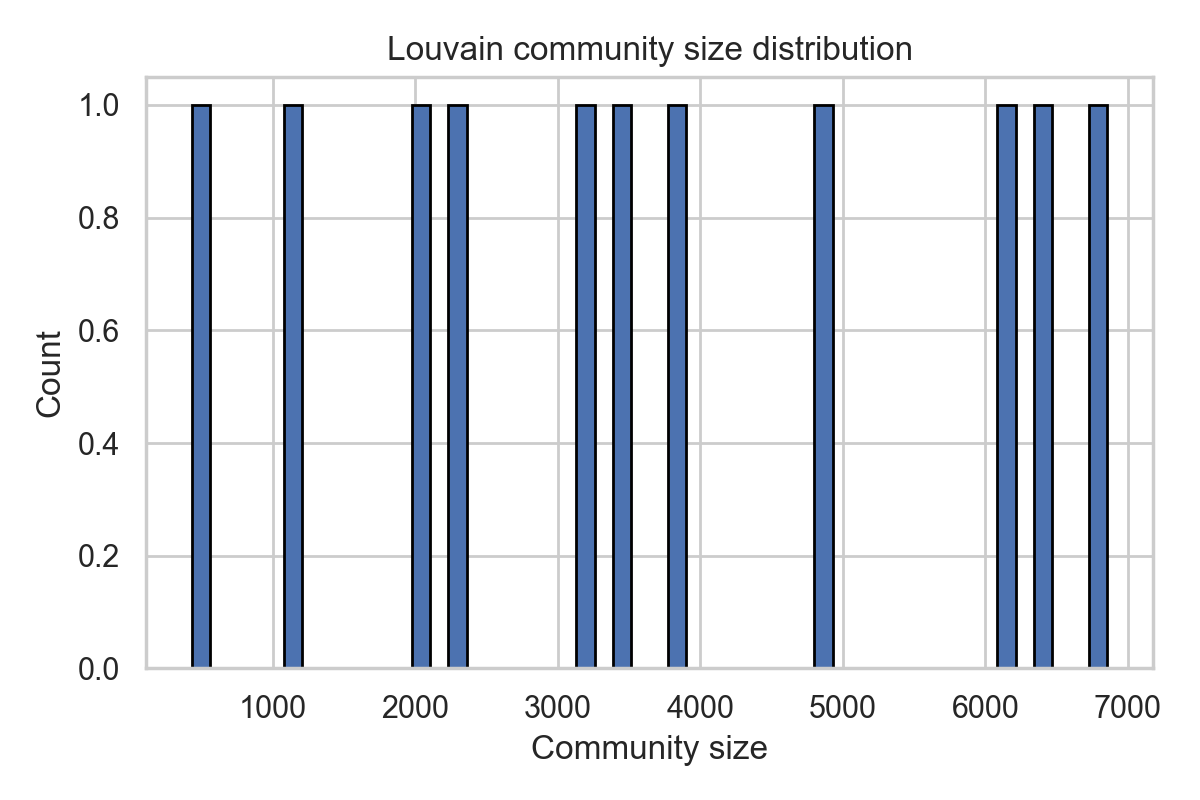
\includegraphics[width=0.48\textwidth]{figures/louvain_community_size_distribution.png}
\caption{Louvain community size distribution.}
\label{fig:louvain_dist}
\end{figure}
\begin{figure}[ht]
\centering
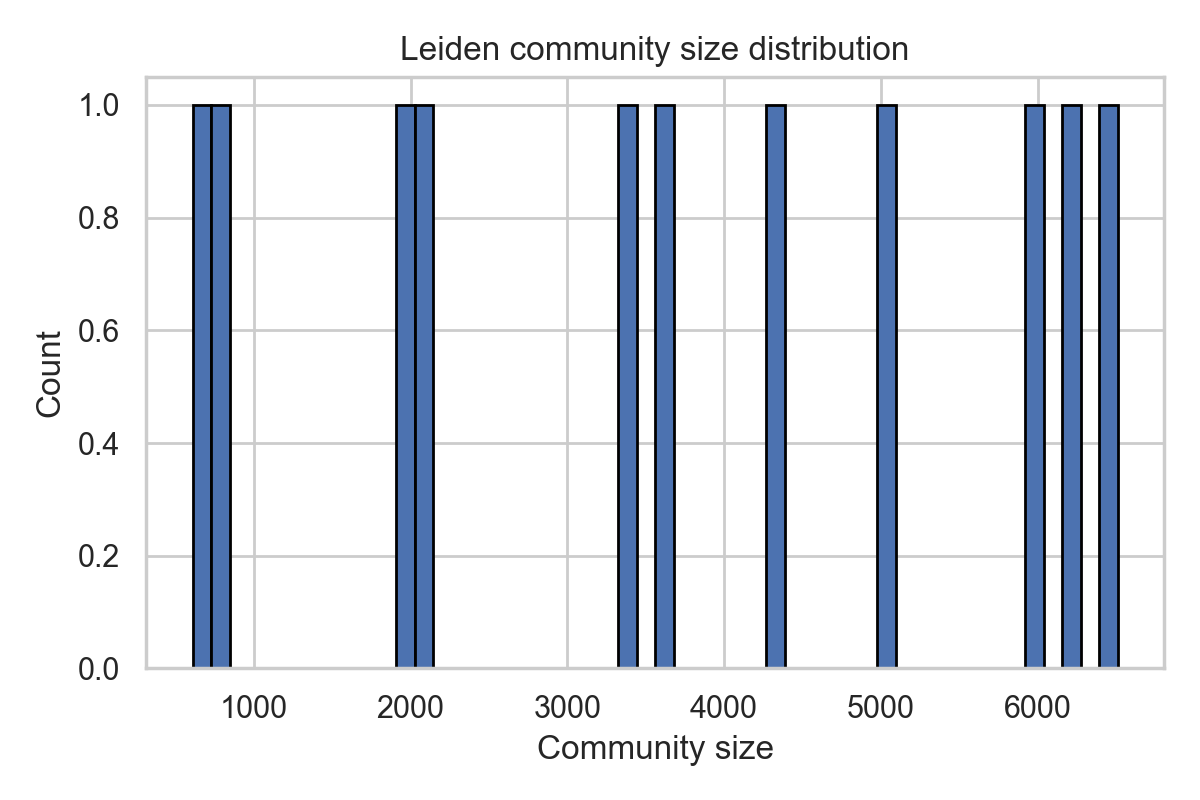
\includegraphics[width=0.48\textwidth]{figures/leiden_community_size_distribution.png}
\caption{Leiden community size distribution.}
\label{fig:leiden_dist}
\end{figure}

\subsection{Representative cliques}
\begin{itemize}
\item \texttt{11972569, 11911591, 12015076, 11996092, 12020388}
\item \texttt{05058140, 00438178, 02058994, 02055975, 00330160}
\item \texttt{12039743, 11556857, 12081022, 12075495}
\item \texttt{11972569, 11911591, 12015076, 11579418}
\item \texttt{02082690, 05088324, 02060141, 07445896}
\item \texttt{01930874, 03244388, 02408281, 03242713}
\item \texttt{01131043, 01549291, 02037272, 02513740}
\item \texttt{00596807, 02984104, 10468559, 10468750}
\item \texttt{15047313, 14603236, 00446329}
\item \texttt{14480772, 00445169, 00445467}
\end{itemize}

\subsection{Discussion}
This section summarizes the robustness and semantic coherence of clusters recovered under tolerance relations. (Add domain-specific discussion here.)